\documentclass{article}
\usepackage{graphicx}
\usepackage{caption}
\newcommand{\HRule}{\rule{\linewidth}{0.5mm}}

\begin{document}

\begin{titlepage}
\begin{center}
\textsc{\LARGE Team2 Inc.}\\[1.5cm]

% title
\HRule \\[1.4cm]
{ \huge \bfseries Ushahidi GeoRole Project Final Report}\\[0.4cm]

\HRule \\[1.5cm]

%Author Data
\begin{minipage}{0.4\textwidth}
\begin{center}
\large Michael Hnatiw, 1684988\\
\large Stephen Lind, 1735827\\
\large Taylor Parrish, 1616044\\
\end{center}
\end{minipage}

%bottom of page
\vfill
{\large \today}
\end{center}
\end{titlepage}

\section{Problem and Resolution}
\subsection{Introduction}
Our changes to Ushahidi implement the ``GeoRole'' functionality outlined in Heather's blog post based on a string matching technique. We envisioned GeoRoles as a method to restrict user reports and administrator verification in order to add credibility and specialization to Ushahidi reports. This system required modification to a variety of controllers, views and models as well as localization modification. The program is ready for a version 1.0 release as all required functionality is present and stable, however there is room is stil room to improve the user experience in future releases.

\section{Accomplishments}
\subsection{Main Map}
\begin{minipage}{\linewidth}
  \centering
  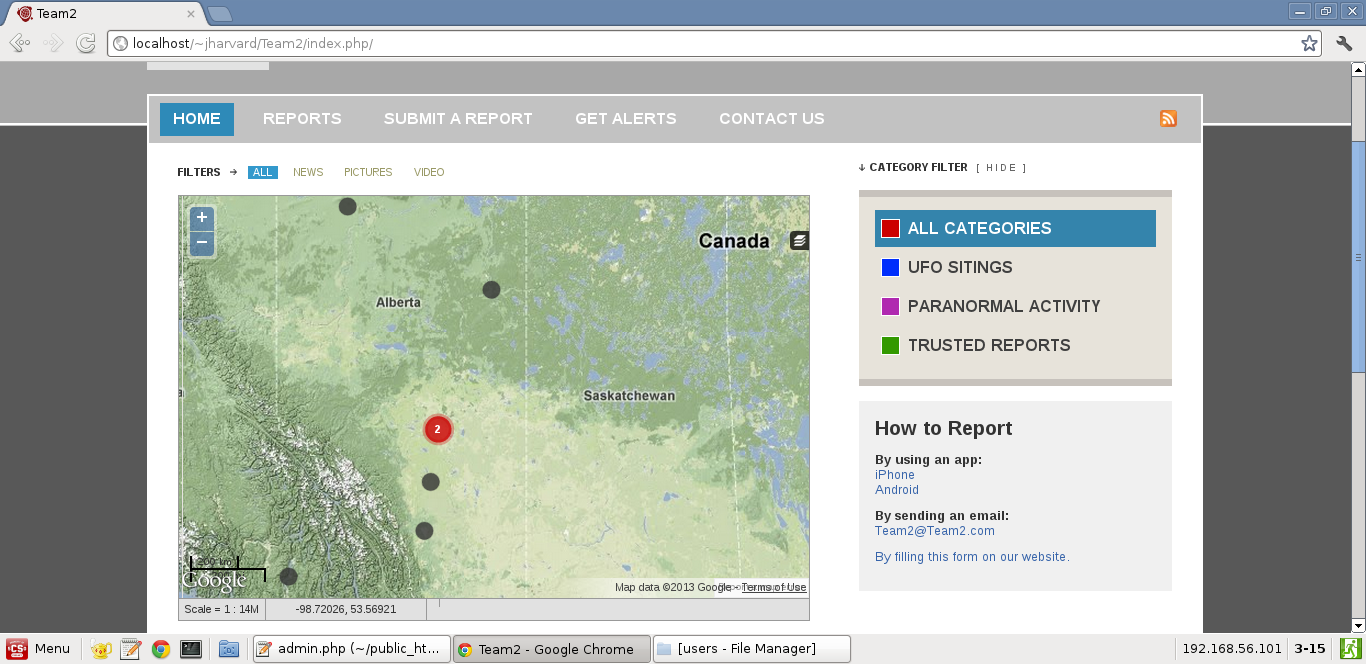
\includegraphics[width=100mm]{mainmapscreen.png}
  \captionof{figure}{Initial User View.}
\end{minipage}
The markers and incidents displayed on the main map are now filtered based on the current users GeoRole. If an incident on the map is within your GeoRole, the incident will show as the color of the category it's in. If it is not, the incident will show as a grey dot.  This incidents are still clickable, but if a user tries to access an incident outside their GeoRole, they will be redirected to the main page and an error will be displayed. 

\subsection{Reports} 
\begin{minipage}{\linewidth}
  \centering
  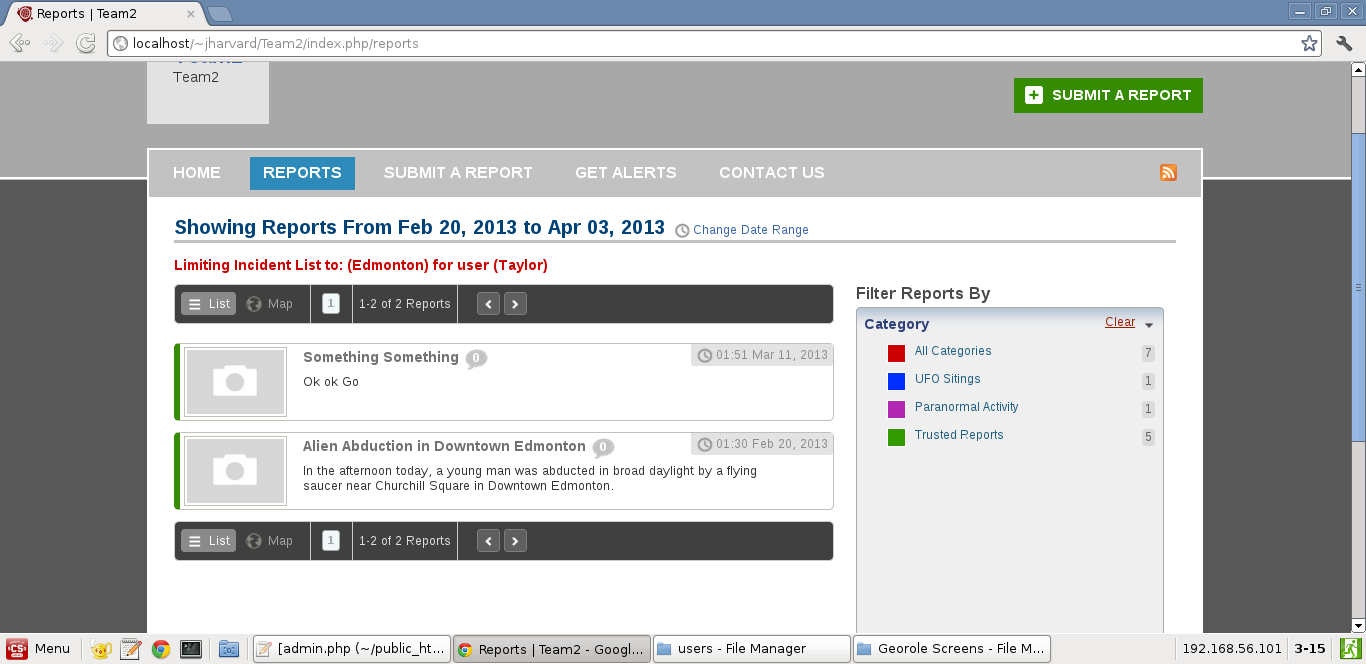
\includegraphics[width=100mm]{reports_list.png}
  \captionof{figure}{Filtered reports list.}
\end{minipage}
The report list is implicitly filtered based on the user's GeoRole. If the user's GeoRole is not specified (ie. NULL) the Reports page will show all reports (A Georole of NULL with a user logged in is given to SUPERADMIN's only).  As well, if no user is logged in (no Georole at all, assumes NULL)  then the viewers of the site will be able to view the full reports list (but as they dont have an account, can not edit or submit reports).  The use of NULL as a base case for restricting access by GeoRole ensures that our version of Ushahidi is backwards compatible with the current official Ushahidi release.
\begin{itemize}
\item \subsection{Submission of Reports}
\begin{minipage}{\linewidth}
  \centering
  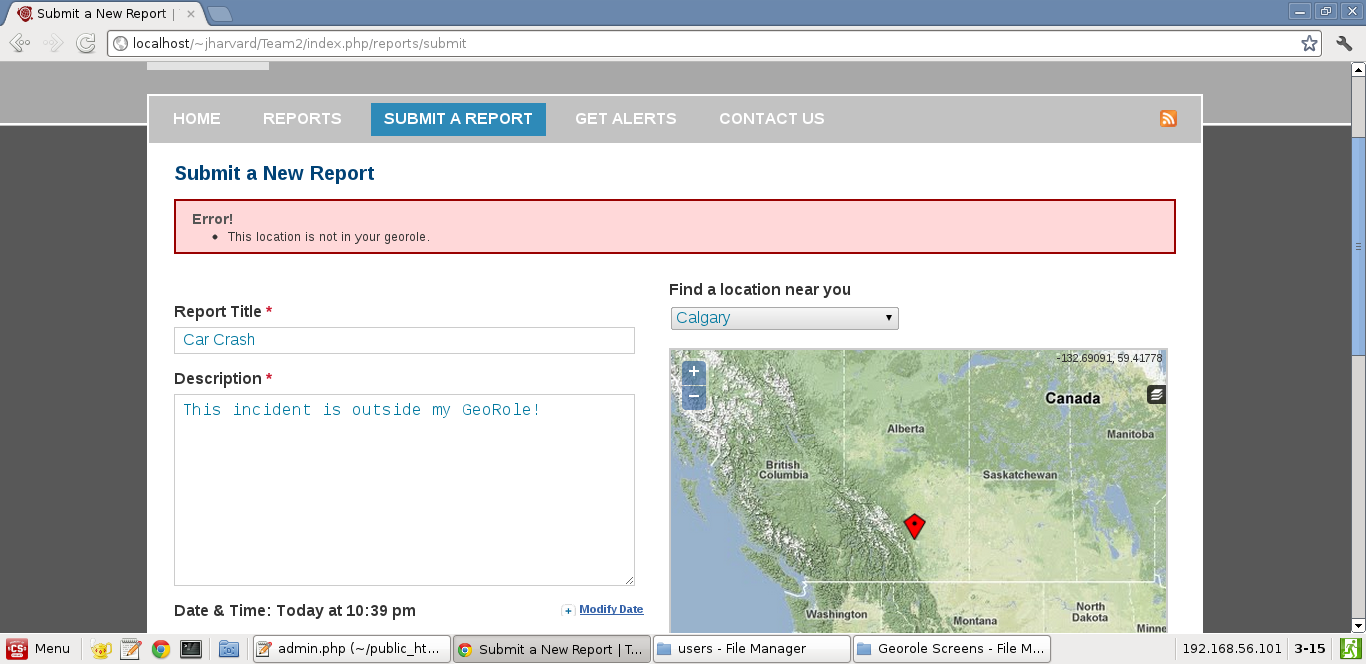
\includegraphics[width=100mm]{submit_report_outside_georole_error.png}
  \captionof{figure}{Error displayed when submitting report outside GeoRole}
\end{minipage}
The submission of a report by a user is also restricted by a users GeoRole.  This prevents users from submitting reports outside their GeoRole.  This helps build the credibility and specialization a GeoRole should provide a user.
\end{itemize}
\begin{itemize}
\item \subsection{Admin Report View}
\begin{minipage}{\linewidth}
  \centering
  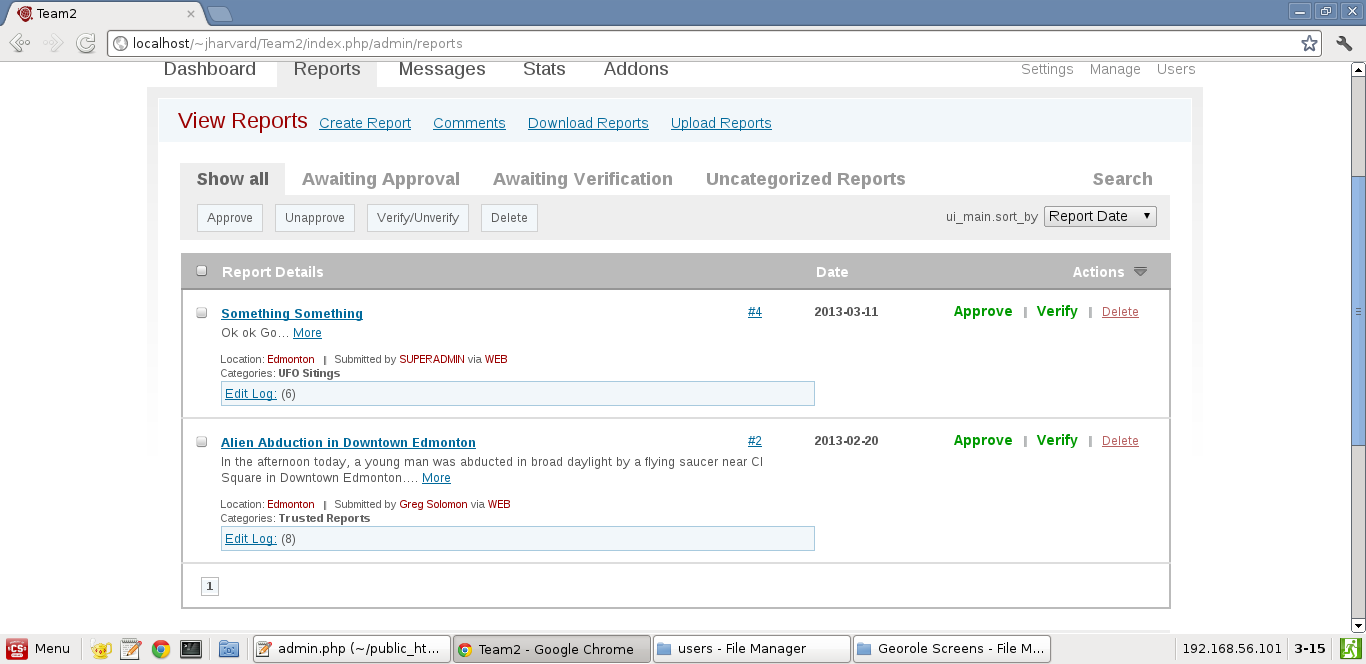
\includegraphics[width=100mm]{admin_dashboard_reports_list.png}
  \captionof{figure}{Administrators View of the Reports List.}
\end{minipage}
The report list on the administrator dashbaord is implictly filtered based on the administrators GeoRole, same as the main report list.  This helps to enforce the user hierarchy as it restricts an admnistrator from viewing and editing (verifying and approving) incidents submitted outside of their GeoRole.
\end{itemize}

\subsection{User List and Hierarchy}
\begin{minipage}{\linewidth}
  \centering
  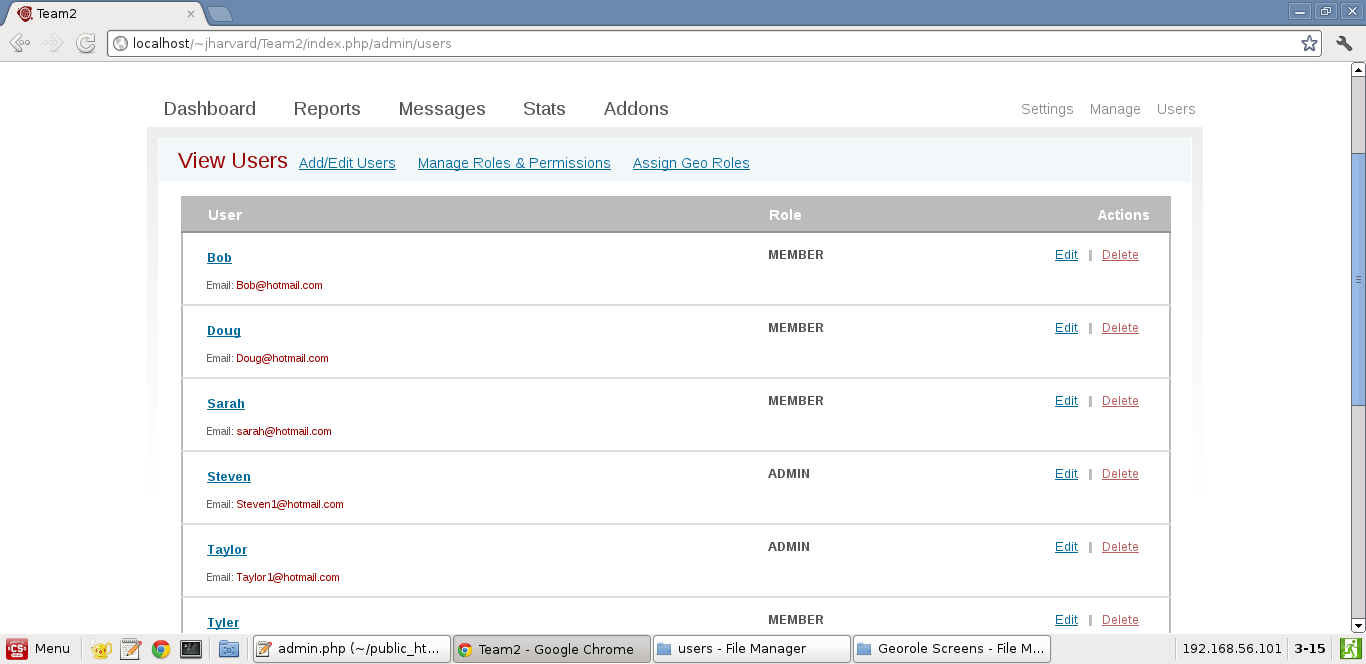
\includegraphics[width=100mm]{user_list.png}
  \captionof{figure}{Administrators View of the Users List.}
\end{minipage}
\begin{minipage}{\linewidth}
  \centering
  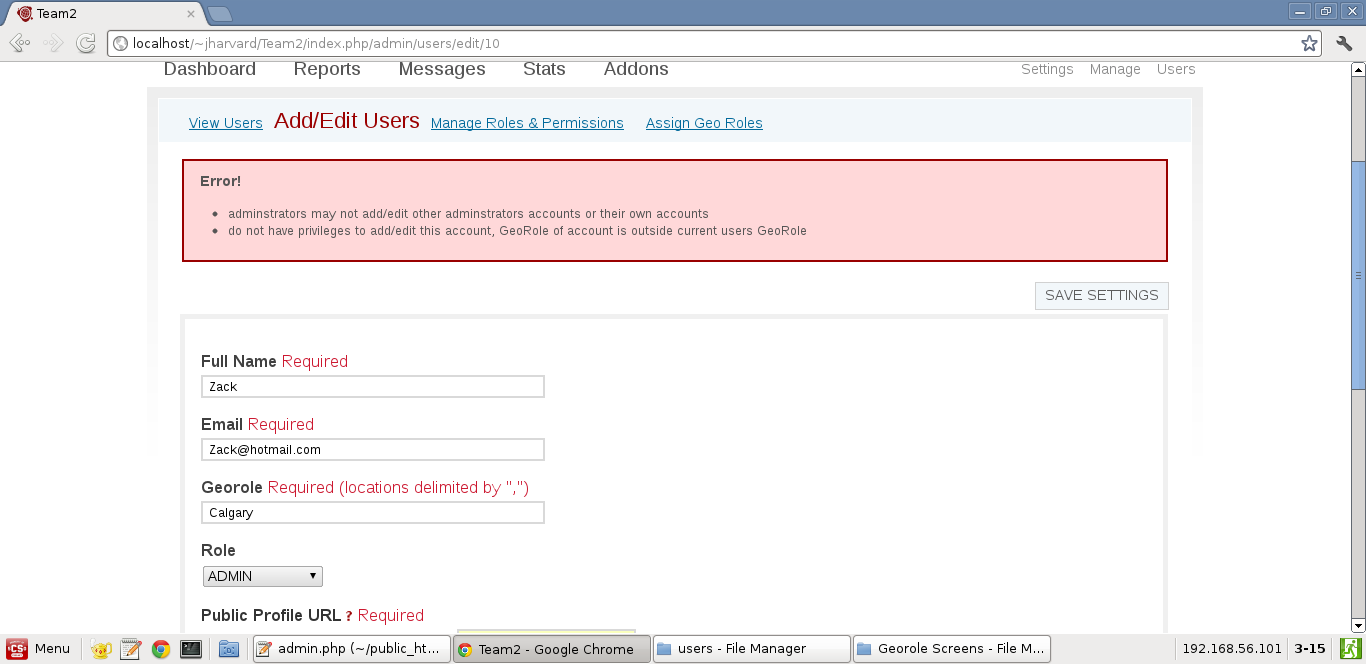
\includegraphics[width=100mm]{multiple_user_list_error.png}
  \captionof{figure}{Various Errors restricting Administrators ability to Edit Accounts.}
\end{minipage}
Administrators implicitly cannot edit users outside of their GeoRole as they are not displayed in the users list on the Admin dashboard. However, other adminsitrators on the system are still displayed to allow adminstrators to coroborate with each other, while at the same time restricting them from editing each others accounts or their own accounts. The SuperAdmin is able to see all users and edit them at a global level, while other user accounts (members and administrators) may not edit nor even view the SuperAdmin's account.  In this way, the user heiarchy is implicitly implemented as administrators may oversee all members within their georole, administrators may share members who have multiple georoles, administrators are restricted from users outside their GeoRole, and the SuperAdmin can oversee all of this having privileges to manage any member or administrator they could want.

\subsection{mySQL Database}
\begin{minipage}{\linewidth}
  \centering
  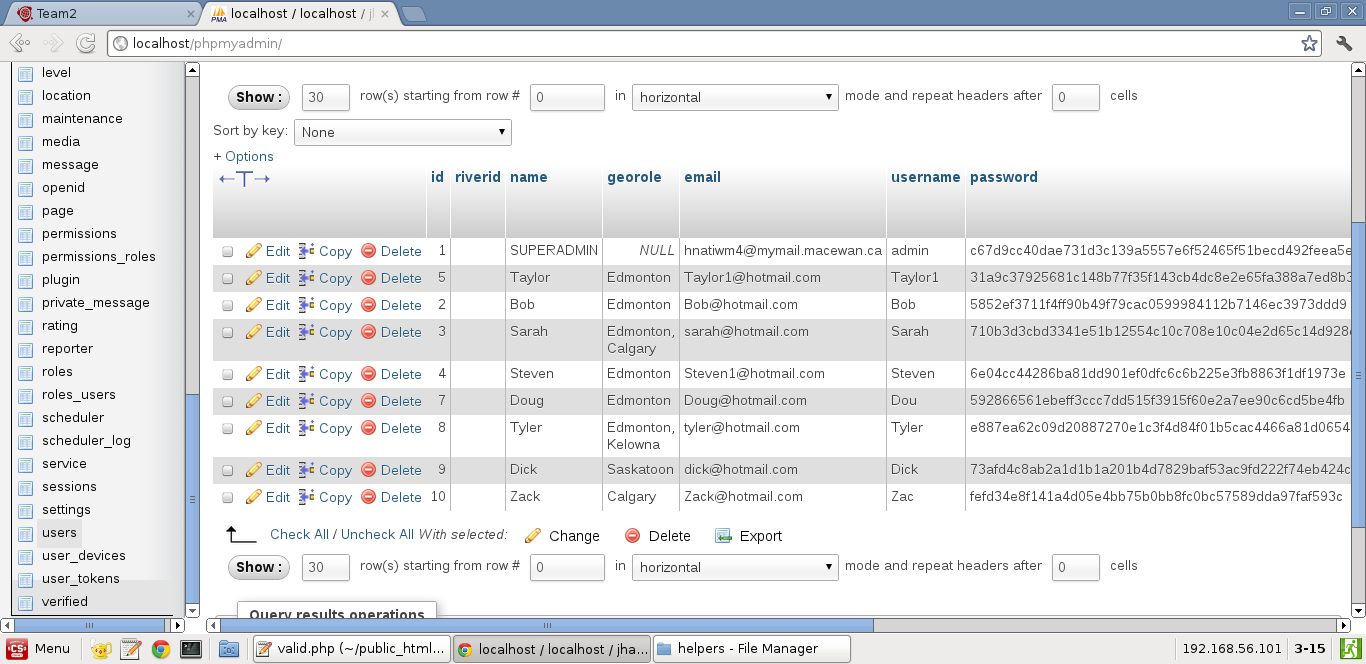
\includegraphics[width=100mm]{sql_table.png}
  \captionof{figure}{Database modifications.}
\end{minipage}
The SQL database was modified to contain a 100 character long field that is used to set GeoRole's based on string comparison.  This was a simple addition that was added to ther Users table.  This allows implementations of Usahidi to enable GeoRoles on t Database side by simply adding a new column to a table in their database.

\section{Tools}
\subsection{JIRA Bug Tracking}
\begin{minipage}{\linewidth}
  \centering
  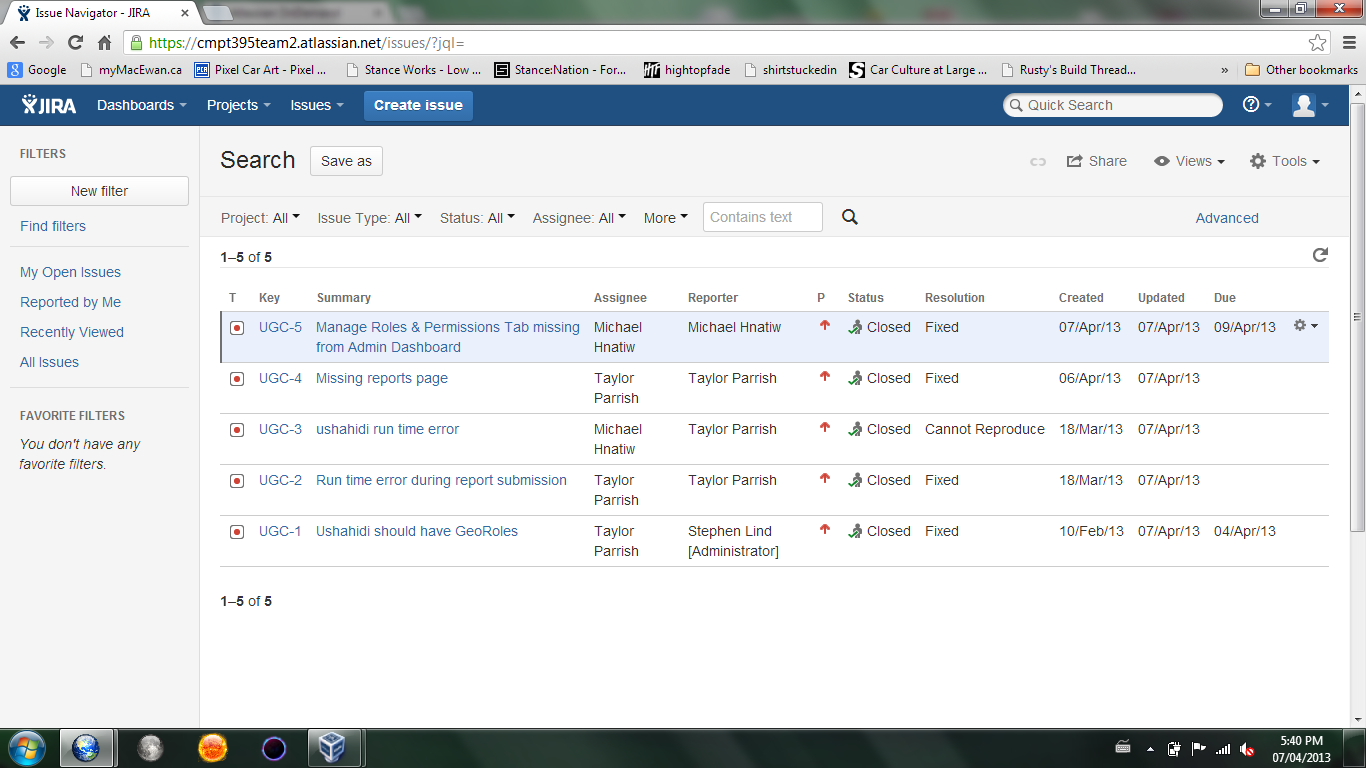
\includegraphics[width=100mm]{jira_bug_list.png}
  \captionof{figure}{Jira Bug List.}
\end{minipage}
For bug tracking we decided to used Jira to track all of our bugs as it allows all our group members to add bugs that are discovered and to allow anyone to resolve them as needed. Most of our bugs were short term and not filed, but anything that took more than a half hour or so were filed, fixed, and closed as needed.

\subsection{GitHub}
GitHub was used as our projects version control. GitHub initially had a steep learning curve and caused some confusion an project version differences among group members, we overall maintained a clean codebase. We eventually settled on branching from develop locally, then rebasing develop and merging the local branch's as our general development procedure. We then merged with master on (some) Mondays as a psuedo weekly build.

\section{Future Versions}
\subsection{Geometry Objects}
One of the project goals was to use a GUI based area selection using a polygon based tool to define a users GeoRole on a more fine grained level than listing cities. We were unable to implement this, and decided to concentrate on ensuring all base functionality and the user hierarchy. This will be the next step for the next version release given the time for one.

\subsection{Installation Procedure}
Currently the database has to be manually altered to add a GeoRole field under the ``User'' relation. This should be set up at install time. Also we would like to implement an installation option for including GeoRoles.

\subsection{Abstraction of Package}
Coupled with the Installation procedure we would like to implement, we would like to abstract all of our work into a seperate package in the name of maintanability and object abstraction. This would clean up our work and ease integration with the main Ushahidi development branch.

\section{Development History}

Feb.11 - Feb.20:

    All of our team members are preoccupied with other class material and course work, as well as the first sprint being dominated by midterms, our plans during reading week have fallen apart.

    We are disorganized but are making progress in understanding Ushahidi's codebase.  No implementation has been decided on as we all work independently trying things out.  Our highest priority goal still is to make the association explicitly defined the a User hiearchy (ie Superadmin-Admin-Member) which is already implemented (may not be want we want though).
		    
    Reading week has turned into experimentation and understanding PHP and Ushahidi's codebase, meaning all the implementation stories for this week must be pushed to the next sprint.

    Although very undesirable, it is expected as out focus factor is very very low due to heavy course and project work in 3 - 4 other classes for all team members (not to mention external responsibities).
	     
    This will be a reoccuring trend of pushing back main stories, but it is still likely we will have a stable implementation or at least prototype by the end of the term.
	
Feb.20 - Feb.23:

    Found a few Kohana tutorials to get a better understanding of the framework.  Most helpful was: http://dev.kohanaframework.org/projects/kohana2/wiki/Kohana101, passed them around to other teammates.

    Found out that view for Submit a New Report page is /Team2/themes/default/views/reports/submit.php
	
Feb.23 - Feb.24:

    Built a simple PHP controller and view for a possible georole creation page, submit button links to the submit page on the Ushahidi instance.
	
    Cant seem to get stylesheet to work correctly inside any view created.
    Seems kohana framework re-routes the link from /~jharvard/kohana/index.php/... to just /kohana/index.php/...
	
Feb.24 - Feb.27:

    Had a quick team meeting in during the CMPT 395 Lab, discussed where we are in terms of understanding the code base and it seems we are still heavily confused.  We are behind alot in terms of what we set out to plan.  All team members have done some kohana and php tutorials to gain a better understanding.
	
    All members have other projects they had to work on so no further work was completed in the lab.

    Overall the team has: 
	***gained better understanind go CSS stylesheet and how php works with HTML***
	***created mockup CreateGeorole webpage in admin dashboard***
	
Feb.28 - Mar.3:

    Discovered that in order to modify the general layout of an interface, need to modify the particular interfaces layout.php file (ex. views/admin/layout.php).
	
    Added code to admin/layout.php on line 235 to test georole.css.
	
Mar.3 - Mar.4:

    GEOMETRY layout from submit report page found in themes/default/views/reports/submit.php, GEOMETRY values from submit report page found in the form[] array object on line 256 of /application/controllers/reports.php and geometries object found in ./default/views/reports/submit_edit_js.php.

    *****drawCircle() function located at line 110 in views/map_common_js	
    *****drawCircle function used in /themes/default/views/reports/reports_js.php

    Discovered that in order to edit anything in any UI, you need to find the applicable .php file in /applications/helpers and then add a string reference in the appropreiate library file in /applications/i18n/en_US/ (ex. ui_admin.php).
	
    *** all text names for all gui objects are dynamically named this way ***

Mar.4 - Mar.5:

    We have divided the tasks among our group members to, at this level:
	
    Michael = read in a georole designated by a name and assign it to the user(is admin level, controler).
    Taylor = when a user tries to submit a report, it validates that it the area is within their georole (just by comparing if their georole is the same as the city in which they are in).
    Stephen = and all the backend database work.

    ****** georoles at this point will just be string values designations cities ******

    Discovered that to add georole proerty, needed to modify or add: 
	 -User_Model in application/models/user.php
	 -added column in database (under users) for georole
         -Need to modify create_user() function definition (add georole) in application/models/user.php
	 -Need to modify create_user() function call in /modules/auth/libraries/drivers/Auth/ORM.php (line 256)
	 -Need to modify create_user() function call in /application/controllers/login.php (line 255)
    
    Successfully adds georole as string to user table in database from /admin/users/edit.php.

Mar.5 - Mar.8:
    
    (Michael) Created two new files to test including a map onto a webpage:
       - applications/controllers/tests/georolemap.php
       - applications/views/tests/georole_map.php
        
    included code from:
       - applications/controllers/admin/reports.php in function edit() starting at line 316
       - applications/views/admin/reports/edit.php on line 203 to 234
        
    Figured out that the GEOMETRY object in the geometry table in database is made up of an SQL GEOMETRY Object (ie contains POINT values) and that the "geometry" variable used in reports.php is made up of an array of values (one for each unique row in the geometry table), and is part of a form object).

Mar.8 - Mar.10:

    No luck with decyphering how graphical geometry control works on applications/views/admin/reports/edit.php page. However, will try to add a custom GeoRole Filter by modifying: /application/controllers/reports.php and /themes/default/views/reports/main.php starting at line 182.

    Will make a controller parse a logged in users georole data, automatically put it into this filter, and restrict list of reports to that location/locations.

Mar. 10 - Mar. 12:

    Report Submission validaiton working with added georole attribute to user model (city must be within users assigned georole before they can submit a report).

    Modified the files: application/helpers/admin.php, application/helpers/reports.php, application/helpers/valid.php, application/libraries/Validation.php, and application/models/user.php
 	   
    Modifying incident.php at line 310 to add to the SQL query, if done right should reduce incidents or reports returned to the list, also modified reports.php at roughly line 1000 to include georole value when passing to fetch_incidents and get_incident functions needed to form query.  However the query is hard to figure out (Michael working on this) so there is no Success so far.
 	     
Mar. 13 - Mar. 14:
            
    Need to find a way to filter the reports list page on the main website layout, to implicitly restrict the list of reports to only incidents reported from a location that corresponds to a users georole, even iffiltered by other fields (ie if choose all categories, still reduces the list).
         
    Made changes to helpers/reports.php and models/incidents.php so that if georole is null, doesnt add line to query so it includes all incidents in list view (default behavior if georole is null is that all reports still added to list in views/reports.php). Implemented function to parse georole and location to match in sql query if georole made of multiple cities.
              
    Added title to reports view page to tell user limiting report list to their georole. Did this by modifying: /themes/default/views/reports/main.php on line 11, /applicaiton/il8n/en_US/ui_main.php on line 196, and /themes/default/css/style.css at end of file.
                
Mar.14 - Mar. 15:
                                
    Modified _get_report_listing_view() function in /controllers/reports.php to recalculate stats_breadcrumb used in report list view to list how many reports are in the list did this by making the function georole_report_count() in the same file (line starting at 206, and function at end of file) fixed georole header message in themes/default/views/reports/main.php to not display is georole is null.
                    
Mar. 15 - Mar. 17:
    
    Implemented function to filter markers based on georole before being rendered as geojson objects. Right now, only renders incidents that are outside a users georole as grey dots, but later want to figure out how to change this to not make incidents clickable by the user).
    
    Modified the file modified applications/controllers/json.php at line 133 and added the function filter_markers() at end of file.
    
    Fixed and cleaned up code created previously in applications/models/incidents.php at line 312 by abstracting code into a function, and removed uneccessary code in applications/helpers/reports.php at end of file.
                
Mar. 17 - Mar. 20:

    ***** Group as a whole decided to scrap the graphical georole implementation we have tried to decypher and implement with the string based one we have been implementing to this point as a safeguard.  We can't seem how to get the values out of the geometry object and store them, nor implant that onto the map and actually restrict the users view of incidents *****

    Everyone created a new local branch and will be working on from that.
    
    Trying to edit report content-block on main map page (small list of incidents under the map) by filtering by the current users georole.  To do this we modified: /applications/il8n/en_Us/ui_main.php at line 197 (added georole_reports_listed) and /themes/default/views/blocks/main_reports.php.
          
    Added a the function filter_incidents() to applications/helpers/blocks.php that takes a georole and incident array and filters the incidents to contain only those within the georole.
 
    Figured out that line 256 in applications/controllers/login.php was causing a runtime error when generating new user (as required georole).  Didn't create a JIRA bug for this as was a quick remedy by removing the unlees code we added to the file when testing things out.
                      
Mar. 20 - Mar.22:

    Couldn't figure out how to make incident markers outside of a users georole, who are now rendered grey, to be non-clickable. So as an alternative, will redirect the user and display an error message when an incident that is outside their current georole is clicked.
    
    Modified /applications/controllers/reports.php at line 470 to redirect the page if a specified incident, that is selected to have its details viewed, are outside a users georole.
    
    Still needs to look at /themes/views/reports/submit.php line 20 to get how the red error box works for the submit page and how to incorporate it into the main page and helpers/report.php at line 38 to get how the error is generated and il8n/en_US/reports.php  for georole how to see where the error messages are.
        
    Modified the files: /themes/default/views/main/layout.php at line 12 to add conditional to show a red error box if current page is the georole_error.php page that copies the main pages session.
            
    Created the file georole_error.php as an exact copy of the Main_Controller class in applications (applicaitons/main.php), except for it displays an error message when a users page is redirected by the due to accessing a georole outside of their georole. This was done becaue simply redirecting the user to the previous page loses the session information so you can't have a controller change a variable in another controller, so we simply create a new session with the same as the one created automatically by Ushahidi and test if the current page is the georole_error page to produce the error message.

Mar. 22 - Mar. 29:

    Discovered that the reports list as has some faults even though reports are filtered the number of pages listed, and the prev and next page buttons to work with the filtered list (in controllers/reports.php in _get_reports_listing function, in helpers/reports.php where pagination object set).
                     
    Modified the files: /applicaitons/helpers/reports.php starting at line 970 to accomidate georole to change pagination and the navigational bar above the reports list and removed stat_breadcrumb change mentioned a few days ago from controllers/reports.php starting at line 195 as changes to helpers now implements what the removed code did.
                       
Mar. 29 - Apr. 4:

    To implicitly restrict an ADMIN user from editing user setting attributes the do not have privileges to edit (ie password, role, georole, etc.) edited /i18n/en_US/ui_admin.php at line 95 to add error messages for admin's trying to edit accounts the shouldn't, /applications/views/admin/users/edit.php at line 20 to display error message if certain flags are set, and add functions to applications/helpers/admin.php at line 309 to compare georoles and to perform checks on the flag (including references the database).  Lastly, edited /controllers/admin/users.php int the function edit() starting at line 85 to incorporate error flags for different conditions, if there set then the changes to the form is never propagated to the DB.
        
    Modifications were succesful at restricting any ADMIN account from editing their own settings and attributes, MEMBER accounts outside their georole, other ADMIN accounts, and any SUPERADMIN account setting and attributes found in the users table in the DB.
                                                                               
Apr. 5 - Apr. 6:

    Introducing authenticaiton when no user is logged in (so the website doesn't crash) introduced a bunch of errors among edited files (due to variables not be defined out of conditionals so if no user logged in, variables dont get values).
            
    Fixed /themes/default/views/reports/list.php at line 26 and 165 (no need to authenticate stats_breadcrumb), applications/controllers/reports.php at line 212 (else statement to set default stats_breadcrumb value) and fixed /applications/helpers/reports.php at the EOF (made function count all roles if georole is NULLfor SUPERADMIN or no logged in)
                
    However, we've encountered a BIG PROBLEM where reports pages are notfound (404 ERROR) if the user has a georole, but are found if no users are logged in or the SUPERADMIN is logged in (georole = NULL). Created a bug report on JIRA (UGC-4). Assigned to Michael and Taylor.
        
Apr. 6 - Apr. 7:

    Still need to implicitly filter user list under admin dashboard to only display users within an admins georole (ie cant see anything outside georole or other administrators).  To do this modified /applicaitons/controllers/admin/user.php at line 71 to filter the user objects by the current users georole using a function, and then changed /applications/helpers/admin.php by adding a function filter_users_on_georole() at line 305 to filter the users object.
    
    However, this didn't produce the desired results as the users object found in /applicaitons/controllers/admin/user.php was not edited when it reached the view, so just ended up adding a conditional to applications/views/admin/users/main.php at line 77 and 133 adds a conditional thats filters any user outside of the current admins georole (keeps all ADMIN accounts in the list).
                
                
    * Resolved resolved page not found issue (JIRA BUG UGC-4) by removing unnecessary conditionals and simply setting a georole variable outside of a loop on page in the reports controller /applicaitions/controllers/reports.php.
      
    Found another bug (UGC-5): Manage Roles & Permissions Tab missing under Admin Dashboard but quickl resolved that by once again removing an unneeded conditional introduced earlier in the view.
            
Apr. 8 - Apr. 9:

    At this point, the implementation has been documented thouroughly, the code has been cleaned up in most places and we have been constantly testing with different user accounts and report cases.  If time allows, we might clean up code even further by placing all the functions in their own helper file.        
 
\vfill
\begin{center}
Project Summary created with la\TeX~.
\end{center}
\end{document}
